%!TEX root = ../main.tex
\chapter{Presentación de resultados}\label{cap:resultados}

El presente capítulo expone los resultados obtenidos en el desarrollo y validación del sistema de facturación automatizada para unidades financiadas, abarcando tanto los resultados favorables como las limitaciones detectadas. Su objetivo es presentar la evidencia de forma objetiva, sin juicios de valor, y vincularla con los objetivos planteados en el Capítulo 1 y con la justificación desarrollada en los Capítulos 4 y 5.

El capítulo se organiza siguiendo el ciclo de desarrollo del prototipo: primero se formalizan los requisitos funcionales y no funcionales; luego se sintetiza el diseño; a continuación, se documenta la construcción e integración con las entidades bancarias; después se describen las pruebas técnicas y de aceptación, junto con el relevamiento realizado con los usuarios del área de cuentas a cobrar; y finalmente se presentan los resultados obtenidos y una síntesis del capítulo.

\section{Requisitos}

Los requisitos surgen del relevamiento del proceso manual descripto en los Capítulos 1 y 4, de las conversaciones con el área de cuentas a cobrar y de las condiciones técnicas impuestas por las APIs de cada entidad bancaria. Se clasifican en funcionales y no funcionales.

La Tabla~\ref{tab:13}

presenta los requisitos funcionales de la solución, indicando para cada uno el país en el que aplica y la aplicación que lo implementa.

\subsection{Requisitos funcionales}

\begin{longtable}[]{@{}
  >{\raggedright\arraybackslash}p{(\columnwidth - 6\tabcolsep) * \real{0.09}}
  >{\raggedright\arraybackslash}p{(\columnwidth - 6\tabcolsep) * \real{0.56}}
  >{\raggedright\arraybackslash}p{(\columnwidth - 6\tabcolsep) * \real{0.15}}
  >{\raggedright\arraybackslash}p{(\columnwidth - 6\tabcolsep) * \real{0.20}}@{}}
\caption{Requisitos funcionales}\label{tab:13}\\
\toprule\noalign{}
\endfirsthead
\caption[]{Requisitos funcionales (continuación)}\\
\toprule\noalign{}
\endhead
\bottomrule\noalign{}
\endlastfoot
ID & Requisito & País & Aplicación \\
RF01 & Consultar automáticamente la línea de crédito disponible de cada concesionario ante la entidad bancaria y actualizar el saldo disponible, reemplazando la carga manual desde el home banking. & Chile y Perú & VH Legacy \\
RF02 & Unificar en la pantalla CR08 la visualización del crédito, separando saldo disponible y facturado para unidades livianas y pesadas (en Perú, solo livianas). & Chile y Perú & VH Legacy \\
RF03 & Permitir la carga masiva de DUA y plazo por VIN mediante un archivo Excel en la pantalla Alta Dua File, con procesamiento batch y notificación por correo del resultado. & Perú & VH Legacy \\
RF04 & Asignar un número de lote a las unidades facturadas en conjunto y registrarlo en la tabla 040\_LOTES\_FACT. & Chile y Perú & VH Legacy \\
RF05 & Detectar, mediante un proceso programado, la finalización de la facturación de un lote y enviar un correo de notificación (correo de despacho) a los usuarios de la empresa (en Chile, además, al equipo de logística, externo a la empresa y a la entidad bancaria, y a Forum), que incluya el número de factura asociado a cada unidad. & Chile y Perú & VH Connect \\
RF06 & Informar a la entidad bancaria las facturas del lote una vez completado: una factura por solicitud en Forum y hasta 25 facturas por solicitud en Santander. & Chile y Perú & VH Connect \\
RF07 & Registrar por VIN la solicitud enviada, la respuesta recibida y el código HTTP de cada transacción en la tabla 055\_TRANSACCIONES\_CREDITO. & Chile y Perú & VH Connect \\
RF08 & Marcar cada unidad como informada al banco mediante las columnas REPORTED\_FORUM y REPORTED\_SANTANDER de 042\_ALTORDEN. & Chile y Perú & VH Connect \\
RF09 & Reenviar automáticamente, mediante un proceso nocturno programado a las 23:00, las unidades rechazadas o pendientes de informar a la entidad bancaria. & Chile y Perú & VH Connect \\
RF10 & Permitir visualizar en la pantalla CR08 el estado de cada unidad rechazada y reenviar manualmente todas las pendientes a Forum, como alternativa a esperar el proceso nocturno. & Chile & VH Legacy \\
\end{longtable}

La Tabla~\ref{tab:14} presenta los requisitos no funcionales, clasificados según la categoría de calidad a la que responden.

\subsection{Requisitos no funcionales}

\begin{longtable}[]{@{}
  >{\raggedright\arraybackslash}p{(\columnwidth - 4\tabcolsep) * \real{0.10}}
  >{\raggedright\arraybackslash}p{(\columnwidth - 4\tabcolsep) * \real{0.62}}
  >{\raggedright\arraybackslash}p{(\columnwidth - 4\tabcolsep) * \real{0.28}}@{}}
\caption{Requisitos no funcionales}\label{tab:14}\\
\toprule\noalign{}
\endfirsthead
\caption[]{Requisitos no funcionales (continuación)}\\
\toprule\noalign{}
\endhead
\bottomrule\noalign{}
\endlastfoot
ID & REQUISITO & CATEGORÍA \\
RNF01 & Las credenciales bancarias no se almacenan en el código: se gestionan en GCP Secret Manager (VH Connect) y en OpenShift (VH Legacy). & Seguridad \\
RNF02 & La autenticación con cada entidad se realiza por token, reutilizado mientras no expire y regenerado automáticamente al vencer o al reiniciar la aplicación. & Seguridad / Disponibilidad \\
RNF03 & Cada intento de comunicación con el banco queda registrado para permitir su auditoría y reproceso. & Trazabilidad \\
RNF04 & Ante un rechazo o error de la entidad bancaria, la unidad conserva el estado de no informada y se reintenta automáticamente en el proceso nocturno de las 23:00; en Chile, además, el usuario puede forzar el reenvío manual sin esperar a ese proceso. & Confiabilidad \\
RNF05 & La solución se integra a la arquitectura existente (VH Legacy, SAI y VH Connect con base Oracle compartida) sin reemplazar componentes preexistentes. & Mantenibilidad \\
RNF06 & Los cambios se promueven por ambientes (dev, qa, prod) mediante ramas en GitHub. & Mantenibilidad \\
RNF07 & Los procesos pesados (carga de DUA, informe al banco) se ejecutan en segundo plano, sin bloquear la navegación del usuario. & Usabilidad / Rendimiento \\
\end{longtable}

\section{Diseño}

El diseño completo de la solución se desarrolló en el Capítulo 4; aquí se resumen únicamente los elementos necesarios para interpretar los resultados.

\begin{itemize}
\item
  La solución extiende una arquitectura preexistente compuesta por tres aplicaciones que comparten una base de datos Oracle: VH Legacy (Java 6 con JavaServer Faces), SAI (capa intermediaria que notifica la legalidad de las facturas) y VH Connect (Java 21 con Spring Boot, exclusivamente backend). El aporte de este trabajo consiste en incorporar la comunicación con las entidades bancarias, que hasta el momento no existía:
\item
  Actualización de crédito: VH Legacy consulta la línea disponible del concesionario ante Forum (Chile) o Santander (Perú) y la refleja en la pantalla CR08 unificada.
\item
  Informe de facturas: VH Connect detecta la finalización de cada lote, notifica por correo a los usuarios y luego informa las facturas a la entidad correspondiente.
\item
  Persistencia y trazabilidad: se incorporan la tabla 055\_TRANSACCIONES\_CREDITO, la tabla 040\_LOTES\_FACT y las columnas REPORTED\_FORUM, REPORTED\_SANTANDER y TVH042\_LOTE en 042\_ALTORDEN.
\end{itemize}

\section{Construcción e integración}

La construcción se realizó de forma incremental sobre el flujo de ramas por ambiente (dev, qa y prod) de GitHub: cada funcionalidad se desarrolló en una rama propia a partir de dev, se integró mediante pull request y luego se promovió a qa y a producción. En las tres aplicaciones (VH Legacy, SAI y VH Connect), cada push a las ramas de dev, qa y producción dispara un despliegue automático en el ambiente correspondiente.

En lugar de mostrar fragmentos de código, esta sección presenta evidencia del funcionamiento del sistema integrado. Se presentan las siguientes figuras:

\begin{enumerate}
\def\labelenumi{\arabic{enumi}.}
\item
  Consulta de línea de crédito de un concesionario y su reflejo en la pantalla CR08 unificada (saldo disponible y facturado, livianos y pesados).
\end{enumerate}

\begin{figure}[H]
\centering
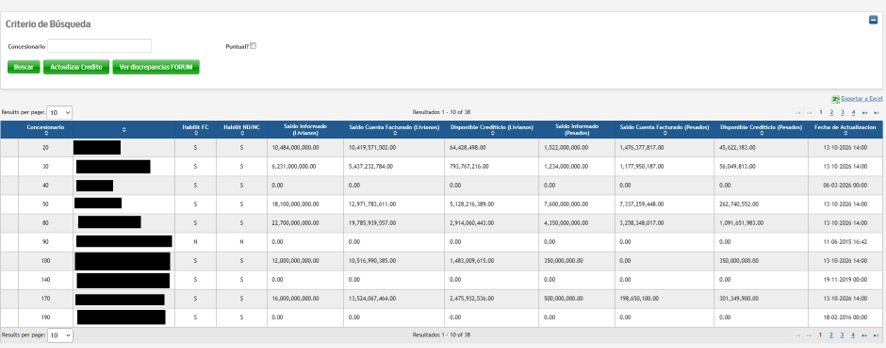
\includegraphics[width=1.00\textwidth]{figuras/image11}
\caption{CR08 de Chile con los saldos de livianos y pesados unificados}\label{fig:10}
\end{figure}

\begin{enumerate}
\def\labelenumi{\arabic{enumi}.}
\setcounter{enumi}{1}
\item
  Pantalla Alta Dua File con la carga de un Excel de ejemplo y el correo de resultado recibido por el usuario.
\end{enumerate}

\begin{figure}[H]
\centering
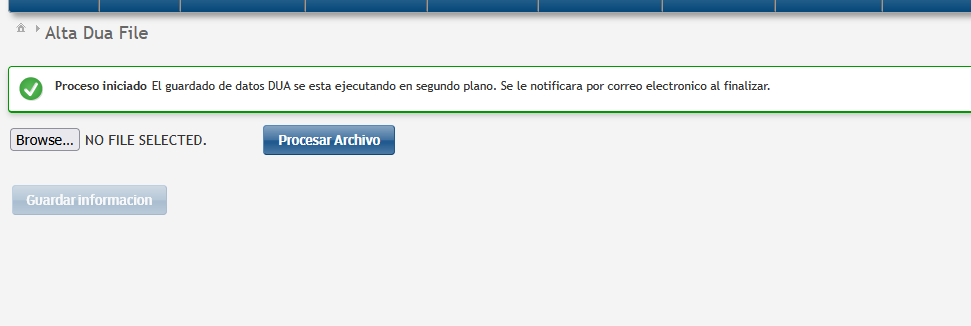
\includegraphics[width=1.00\textwidth]{figuras/image12}
\caption{Pantalla Alta Dua File para cargar el Excel con DUA}\label{fig:11}
\end{figure}

\begin{figure}[H]
\centering
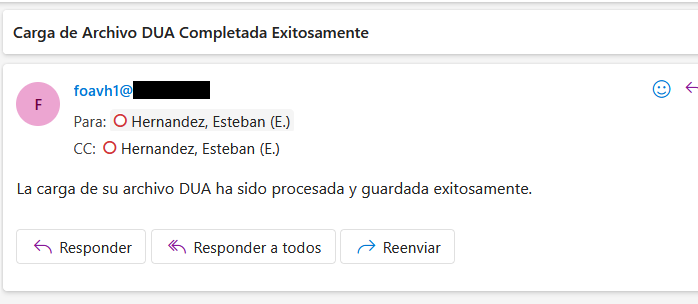
\includegraphics[width=1.00\textwidth]{figuras/image13}
\caption{Correo de confirmación de DUA completo}\label{fig:12}
\end{figure}

\begin{enumerate}
\def\labelenumi{\arabic{enumi}.}
\setcounter{enumi}{2}
\item
  Registros de la tabla 055\_TRANSACCIONES\_CREDITO para un conjunto de VIN, mostrando request, response y código HTTP.
\end{enumerate}

\begin{figure}[H]
\centering
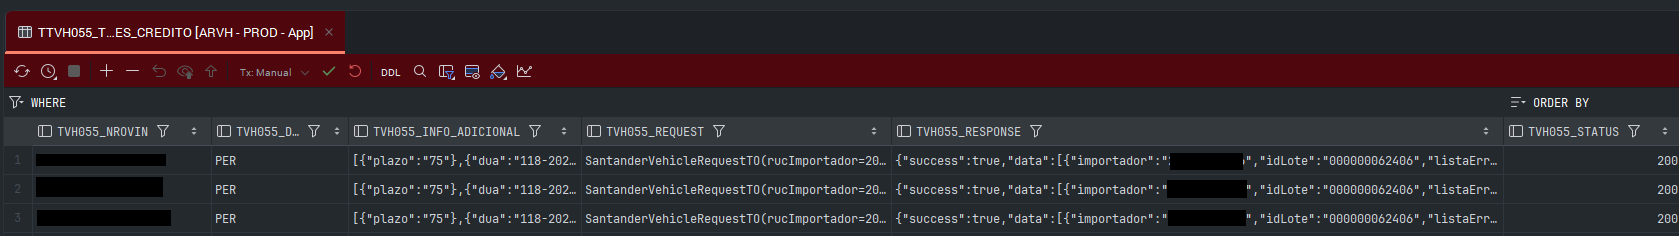
\includegraphics[width=1.00\textwidth]{figuras/image14}
\caption{Datos cargados luego de subir el archivo}\label{fig:13}
\end{figure}

\begin{enumerate}
\def\labelenumi{\arabic{enumi}.}
\setcounter{enumi}{3}
\item
  Correo de despacho recibido por los usuarios de la empresa (ver Validación durante el diseño).
\item
  Registro de 042\_ALTORDEN con las columnas REPORTED\_FORUM / REPORTED\_SANTANDER actualizadas tras el informe al banco.
\end{enumerate}

\begin{figure}[H]
\centering
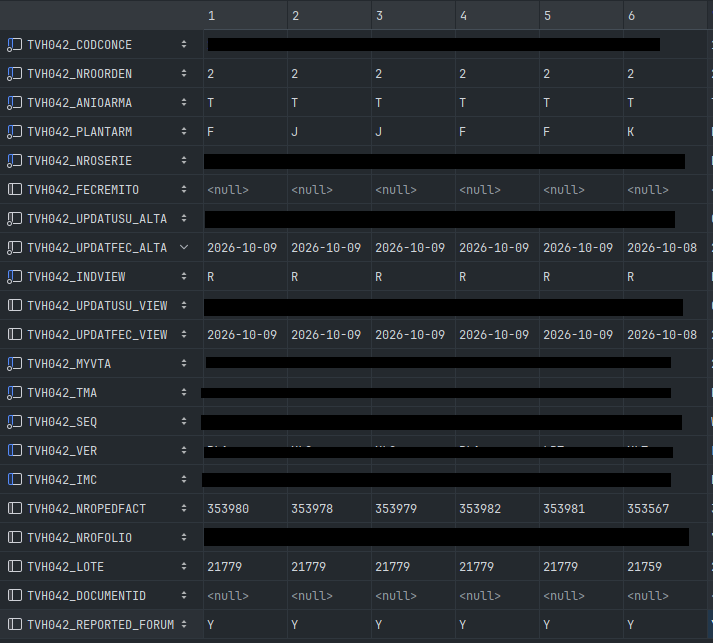
\includegraphics[width=1.00\textwidth]{figuras/image15}
\caption{Status REPORTED\_FORUM en Y (enviado OK)}\label{fig:14}
\end{figure}

\begin{figure}[H]
\centering
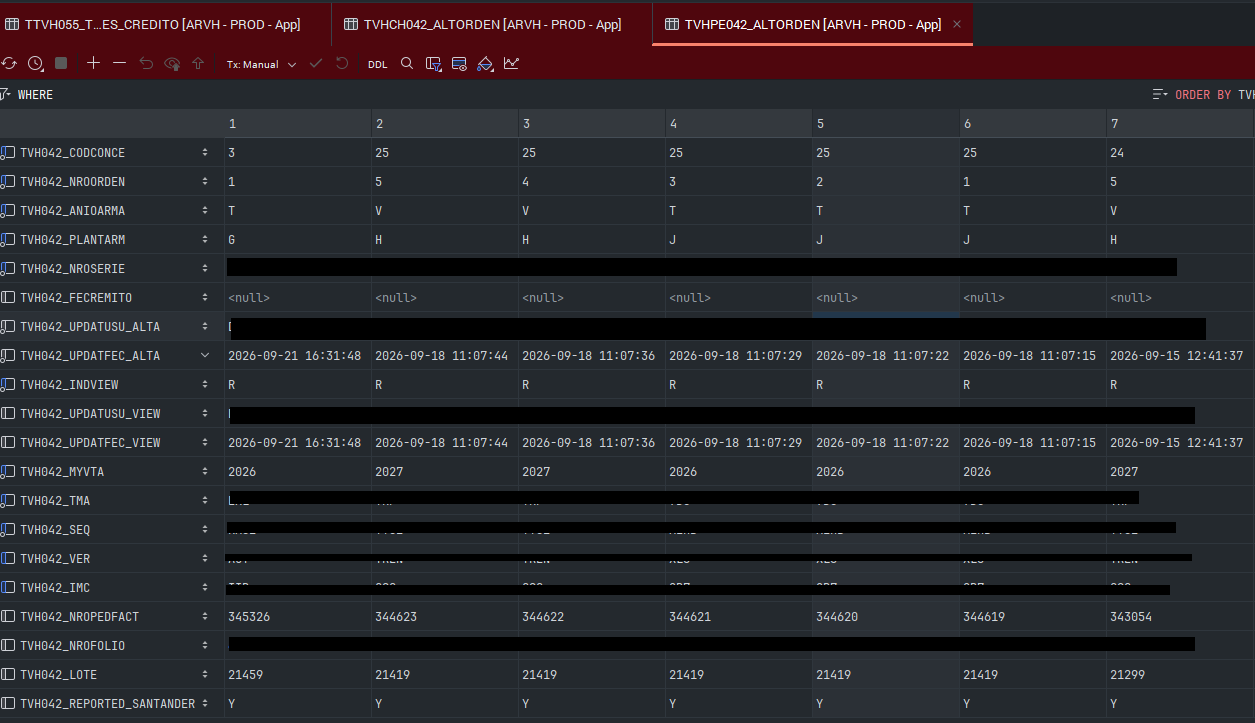
\includegraphics[width=1.00\textwidth]{figuras/image16}
\caption{Status REPORTED\_SANTANDER en Y (enviado OK)}\label{fig:15}
\end{figure}

Uno de los desafíos de integración fue la convivencia de dos plataformas tecnológicas muy distintas. La autenticación por token se implementó con el mismo mecanismo en VH Legacy (Java 6) y en VH Connect (Java 21), aunque con implementaciones diferentes por las limitaciones de la versión de Java de la aplicación legada. Además, cada entidad presenta su propio contrato: Santander recibe las credenciales en el cuerpo JSON de la solicitud, mientras que Forum las recibe como parámetros de encabezado.

\subsection{Problemas detectados durante la integración}

Durante la implementación y las validaciones en producción surgieron errores que no eran previsibles a partir de la documentación de las entidades. Se registran en la Tabla~\ref{tab:15} porque constituyen resultados del trabajo tan relevantes como los casos exitosos.

\begin{longtable}[]{@{}
  >{\raggedright\arraybackslash}p{(\columnwidth - 8\tabcolsep) * \real{0.20}}
  >{\raggedright\arraybackslash}p{(\columnwidth - 8\tabcolsep) * \real{0.12}}
  >{\raggedright\arraybackslash}p{(\columnwidth - 8\tabcolsep) * \real{0.24}}
  >{\raggedright\arraybackslash}p{(\columnwidth - 8\tabcolsep) * \real{0.20}}
  >{\raggedright\arraybackslash}p{(\columnwidth - 8\tabcolsep) * \real{0.24}}@{}}
\caption{Problemas detectados durante la integración}\label{tab:15}\\
\toprule\noalign{}
\endfirsthead
\caption[]{Problemas detectados durante la integración (continuación)}\\
\toprule\noalign{}
\endhead
\bottomrule\noalign{}
\endlastfoot
\textbf{Problema} & \textbf{Entidad} & \textbf{Causa} & \textbf{Impacto} & \textbf{Corrección} \\
Precio de la factura interpretado con la coma desplazada & Santander (Perú) & La documentación no especificaba que el importe debía enviarse siempre con dos decimales. Cuando el precio terminaba en cero se enviaba con un solo decimal, y la entidad interpretaba los dos últimos dígitos como centavos. & Un importe de 28123,10 se registraba en Santander como 2812,31. & Se ajustó el formato para enviar siempre el importe con dos decimales. \\
Fallo de conexión segura desde VH Legacy & Santander (Perú) & VH Legacy no contaba con el certificado SSL de la entidad, necesario para establecer la conexión HTTPS. & VH Legacy no podía comunicarse con la entidad y la consulta de líneas de crédito fallaba. & Se incorporó el certificado de la entidad a uno de los almacenes de certificados (JKS/P12) utilizados por la aplicación. \\
\end{longtable}

Estos casos muestran una limitación habitual en las integraciones con terceros: la documentación de la API no siempre refleja todas las reglas de validación ni los requisitos de conexión de la entidad, y algunas solo se descubren al operar con datos reales. En el caso de Santander, la ausencia de un ambiente de pruebas hizo que el error de formato se detectara recién en producción.

\section{Pruebas técnicas}

Las pruebas técnicas se organizaron en dos niveles: pruebas unitarias automatizadas sobre VH Connect y pruebas de integración contra los servicios de cada entidad bancaria.

\subsection{Pruebas unitarias}

VH Connect cuenta con un conjunto de pruebas unitarias desarrolladas con JUnit, que validan de forma aislada los componentes de la aplicación incorporados en este trabajo. Estas pruebas permiten detectar regresiones durante el desarrollo, antes de que los cambios se promuevan entre ambientes. VH Legacy, por su parte, no dispone de pruebas automatizadas, por lo que sus modificaciones se validaron manualmente en el ambiente de qa.

\subsection{Pruebas de integración con las entidades bancarias}

Las condiciones de prueba difieren entre países. Forum (Chile) dispone de ambientes de desarrollo y producción, lo que permitió validar la integración sin afectar datos reales. Santander (Perú), en cambio, solo expone un ambiente productivo, por lo que las pruebas debieron realizarse directamente sobre producción con un alcance controlado. Para mitigar el riesgo de esta modalidad, las primeras pruebas se coordinaron con el usuario de Perú responsable de aprobar las planillas en el home banking de Santander: el autor enviaba solicitudes con unidades de prueba y el usuario las rechazaba desde el home banking, de modo que se validaba la comunicación con la entidad y la recepción correcta de la información sin generar desembolsos reales.

La Tabla~\ref{tab:16} resume los escenarios probados en cada entidad, el ambiente utilizado y el resultado obtenido.

\begin{longtable}[]{@{}
  >{\raggedright\arraybackslash}p{(\columnwidth - 6\tabcolsep) * \real{0.3912}}
  >{\raggedright\arraybackslash}p{(\columnwidth - 6\tabcolsep) * \real{0.1947}}
  >{\raggedright\arraybackslash}p{(\columnwidth - 6\tabcolsep) * \real{0.2053}}
  >{\raggedright\arraybackslash}p{(\columnwidth - 6\tabcolsep) * \real{0.2088}}@{}}
\caption{Pruebas de integración con las entidades bancarias}\label{tab:16}\\
\toprule\noalign{}
\endfirsthead
\caption[]{Pruebas de integración con las entidades bancarias (continuación)}\\
\toprule\noalign{}
\endhead
\bottomrule\noalign{}
\endlastfoot
\textbf{Escenario} & \textbf{Entidad} & \textbf{Ambiente} & \textbf{Resultado} \\
Obtención de token y consulta de línea de crédito & Forum & Pruebas y producción & Satisfactorio \\
Obtención de token y consulta de línea de crédito & Santander & Producción & Satisfactorio \\
Reutilización de token vigente y regeneración al expirar & Forum / Santander & Pruebas y producción & Satisfactorio \\
Informe de facturas (una por solicitud) & Forum & Pruebas & Satisfactorio \\
Informe de un lote de facturas (hasta 25 por solicitud) & Santander & Producción, lote reducido & Satisfactorio con observaciones \\
Rechazo por datos inválidos y registro en 055\_TRANSACCIONES\_CREDITO & Forum / Santander & Pruebas y producción & Satisfactorio \\
Reenvío de rechazados en el proceso nocturno & Forum / Santander & Pruebas y producción & Satisfactorio \\
Detección de lote completo y envío del correo de despacho & --- & Pruebas y producción & Satisfactorio \\
\end{longtable}

La ausencia de un ambiente de pruebas en Santander constituye una limitación relevante: restringe la cantidad de escenarios de error que pueden reproducirse sin riesgo y obliga a validar ciertos comportamientos recién en producción.

\section{Pruebas de aceptación y relevamiento con usuarios}

Los usuarios del flujo pertenecen al área de cuentas a cobrar de Argentina, que tiene a su cargo también la operación de Chile y Perú. Su participación se dio en dos momentos: durante el diseño, a través de conversaciones informales, y durante la validación, mediante demostraciones del flujo en ambiente de pruebas y validaciones controladas en producción.

\subsection{Validación durante el diseño}

La unificación de las pantallas CR08 y CR12 surgió de una conversación informal y presencial con el equipo de cuentas a cobrar. Hasta entonces, CR08 mostraba el crédito de unidades pesadas y CR12 el de unidades livianas, y no existía forma automática de saber qué concesionarios operaban con ambos tipos. A partir de ese intercambio se optó por concentrar toda la información en CR08. Del mismo modo, el requerimiento de un correo automático al completarse la facturación de un lote surgió de los usuarios, que hasta entonces debían revisar repetidamente el estado de las unidades en VH Legacy.

Cabe señalar que esta validación fue informal y no quedó registrada con un instrumento estructurado, lo que constituye una limitación metodológica.

La participación de los usuarios continuó una vez presentada la solución. Tras conocer el correo de despacho, que se envía al completarse un lote, el equipo de cuentas a cobrar solicitó por correo electrónico, el 9 de septiembre de 2026, que se incluyera el número de factura asociado a cada unidad facturada, de modo de poder identificar cada operación sin consultar VH Legacy. Este pedido se incorporó como ajuste al requerimiento original y evidencia que el contacto con los usuarios permitió refinar la solución de forma iterativa.

Las Figuras~\ref{fig:16} a ~\ref{fig:18} muestran esta evolución: el correo que se enviaba manualmente para notificar las unidades facturadas, la solicitud del usuario y la primera versión del correo de despacho automático.

\begin{figure}[H]
\centering
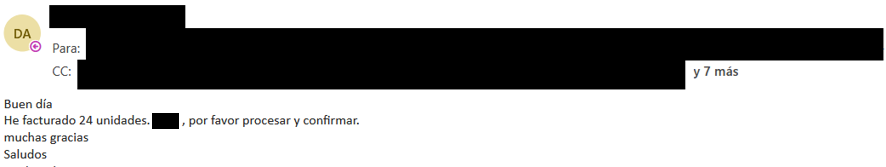
\includegraphics[width=1.00\textwidth]{figuras/image17}
\caption{Correo manual utilizado para notificar las unidades facturadas, previo a la implementación del correo de despacho}\label{fig:16}
\end{figure}

\begin{figure}[H]
\centering
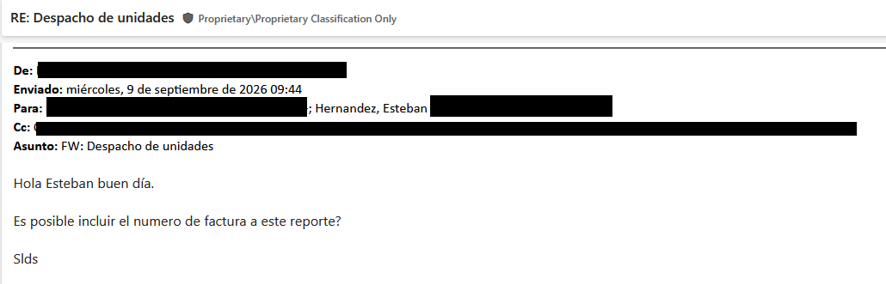
\includegraphics[width=1.00\textwidth]{figuras/image18}
\caption{Correo del usuario solicitando incorporar el número de factura al correo de despacho}\label{fig:17}
\end{figure}

\begin{figure}[H]
\centering
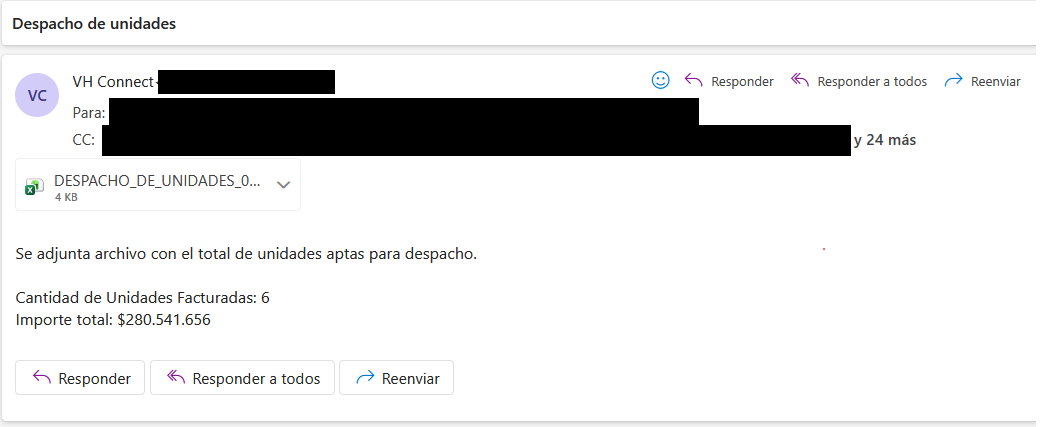
\includegraphics[width=1.00\textwidth]{figuras/image19}
\caption{Correo de despacho previo al ajuste, sin el número de factura por unidad}\label{fig:18}
\end{figure}

A partir de esta solicitud, el correo de despacho pasó a incluir el número de factura de cada unidad.

\subsection{Pruebas de aceptación}

La estrategia de validación se adaptó al riesgo de cada funcionalidad y a los ambientes disponibles en cada entidad bancaria:

\begin{itemize}
\item
  \textbf{Actualización de líneas de crédito (CR08, Chile y Perú)}: la funcionalidad se mostró a los usuarios en el ambiente de pruebas y luego se implementó en producción para verificar la comunicación real con las entidades. Al tratarse de APIs de consulta, que no modifican información en el banco, su validación en producción no implicaba riesgo.
\item
  \textbf{Informe de facturas a Forum (Chile)}: se realizó una demostración en el ambiente de pruebas de la entidad, sin inconvenientes.
\item
  \textbf{Informe de facturas a Santander (Perú)}: dado que la entidad no ofrece un ambiente de pruebas, la validación se realiza en producción con un lote reducido de unidades, para verificar que la información fluya correctamente sin exponer un volumen significativo de operaciones.
\end{itemize}

La Tabla~\ref{tab:17} detalla los criterios de aceptación evaluados, el ambiente en que se validó cada uno y su resultado.

\begin{longtable}[]{@{}
  >{\raggedright\arraybackslash}p{(\columnwidth - 8\tabcolsep) * \real{0.30}}
  >{\raggedright\arraybackslash}p{(\columnwidth - 8\tabcolsep) * \real{0.14}}
  >{\raggedright\arraybackslash}p{(\columnwidth - 8\tabcolsep) * \real{0.12}}
  >{\raggedright\arraybackslash}p{(\columnwidth - 8\tabcolsep) * \real{0.14}}
  >{\raggedright\arraybackslash}p{(\columnwidth - 8\tabcolsep) * \real{0.30}}@{}}
\caption{Criterios de aceptación y resultados}\label{tab:17}\\
\toprule\noalign{}
\endfirsthead
\caption[]{Criterios de aceptación y resultados (continuación)}\\
\toprule\noalign{}
\endhead
\bottomrule\noalign{}
\endlastfoot
\textbf{Criterio de aceptación} & \textbf{Operación} & \textbf{Ambiente} & \textbf{Resultado} & \textbf{Observaciones} \\
El saldo disponible se actualiza en CR08 sin ingresar al home banking & Chile y Perú & Pruebas y producción & Satisfactorio & API de consulta, sin riesgo sobre datos del banco \\
CR08 muestra correctamente saldos de livianos y pesados & Chile y Perú & Pruebas & Satisfactorio & \\
Las facturas se informan a Forum sin intervención manual & Chile & Pruebas (Forum) & Satisfactorio & Sin inconvenientes en la demo \\
Las facturas se informan a Santander sin intervención manual & Perú & Producción, lote reducido & Satisfactorio con observaciones & Validación controlada por falta de ambiente de pruebas. Se detectó el error de formato en los importes (ver Problemas detectados durante la integración), que fue corregido. \\
Alta Dua File procesa el Excel y notifica errores & Perú & Pruebas y producción & Satisfactorio & \\
Se recibe el correo al completarse un lote & Chile y Perú & Pruebas y producción & Satisfactorio & A pedido de los usuarios se incorporó el número de factura por unidad (ver Validación durante el diseño). \\
\end{longtable}

\subsection{Entrevista a usuarios referentes}

Para complementar las validaciones funcionales, se realizaron entrevistas semiestructuradas a dos usuarios clave del proceso. El primero es un integrante del equipo de cuentas a cobrar que actuó como referente durante todo el proyecto: fue el principal contacto para relevar el proceso manual, organizar reuniones con el área y validar los requerimientos. El segundo es un integrante del área de Gerencia de Ventas vinculado a la operación de Perú, que interviene en la carga de los datos de DUA y es responsable de aprobar o rechazar en el home banking de Santander las planillas enviadas para el desembolso, por lo que conoce en detalle la operación de ese país. En conjunto, ambos permiten evaluar el cambio desde la operación de Chile y de Perú.

Las entrevistas se realizaron el martes 6 de octubre de 2026, en forma presencial con el primer entrevistado, y el jueves 8 de octubre de 2026, por videollamada con el segundo, y abordaron cuatro ejes: la situación previa, los tiempos del proceso, la calidad y confiabilidad de la información, y la experiencia de uso de la nueva solución.

\textbf{Situación previa.} El usuario referente señaló que en Chile la carga de crédito dependía de que los analistas de ese país enviaran por correo la información de las líneas disponibles, en formato de imagen. Esto obligaba a transcribir cada saldo manualmente: ``\emph{Al enviar una imagen, se debía cargar cada línea de crédito a ojo}''. Además, cuando un concesionario tenía líneas de livianos y pesados, la carga debía hacerse en dos pantallas distintas. En Perú el proceso era más simple, ya que se maneja una sola línea de crédito (livianos) y se trabaja con pocos concesionarios. La información se obtenía desde el home banking de la entidad, cuando el usuario contaba con acceso, o se recibía por correo en caso contrario. Este relato precisa la descripción del proceso realizada en capítulos anteriores: en Chile, al riesgo de transcripción se sumaba la dependencia de un tercero para obtener la información.

\begin{figure}[H]
\centering
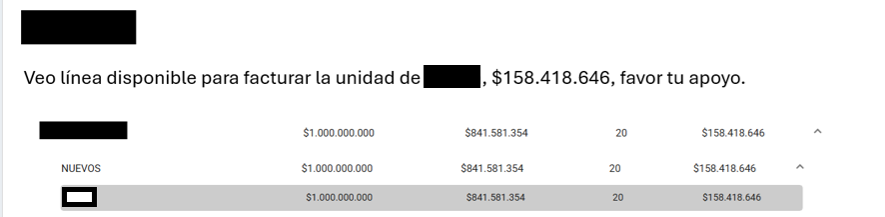
\includegraphics[width=1.00\textwidth]{figuras/image20}
\caption{Correo con la línea de crédito disponible de un concesionario de Chile, previo a la integración}\label{fig:19}
\end{figure}

\begin{figure}[H]
\centering
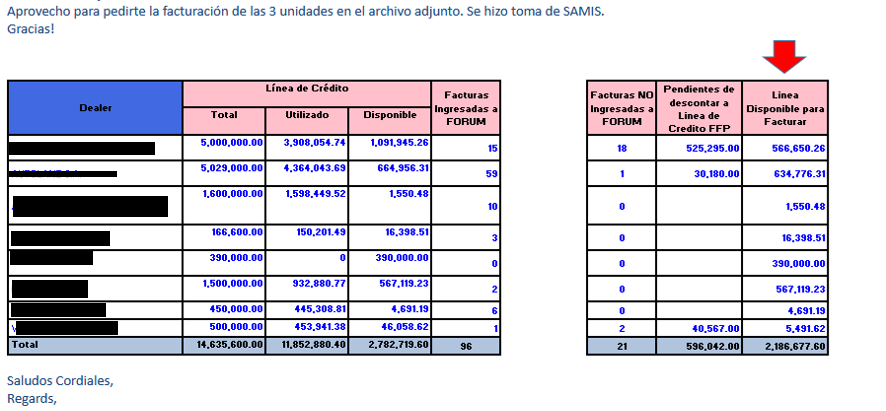
\includegraphics[width=1.00\textwidth]{figuras/image21}
\caption{Correo con el detalle de líneas de crédito por concesionario de Perú, previo a la integración}\label{fig:20}
\end{figure}

\textbf{Tiempos.} El usuario referente no precisó un tiempo por concesionario, ya que este variaba según el momento del mes y la cantidad de unidades. Indicó que el cierre de mes concentra la mayor carga de facturación, aunque también hay picos a mitad o principio de mes cuando no se logra facturar todo en el cierre. En términos globales, afirmó que ``\emph{se llega a perder horas semanales}'', una apreciación consistente con la estimación del Capítulo 5 (aproximadamente 442 horas anuales, equivalentes a unas 8,5 horas por semana). Con la solución, la actualización del saldo se realiza \emph{``en segundos''}. Por su parte, el usuario de Perú confirmó que el armado del Excel para Santander dependía de la cantidad de unidades facturadas y podía superar los diez minutos por concesionario, ya que debía cargarse el precio, la fecha de factura y los datos aduaneros de cada vehículo, con un archivo distinto por concesionario.

\textbf{Errores y confiabilidad.} El usuario referente confirmó la ocurrencia de errores de carga, especialmente en Chile, donde los saldos se expresan en millones de pesos y pueden superar las diez cifras: \emph{``Muy común olvidarse de poner un 0 y, por ejemplo, en vez de tener un saldo disponible de 1.000.000.000 era 100.000.000''}. Estos errores interrumpían la facturación por saldo insuficiente y obligaban a investigar la causa y recalcular el saldo faltante, y eran más frecuentes en los cierres, \emph{``donde se trabajó todo el día y capaz se continúa facturando a las 11 de la noche''}. Sobre la solución, consideró que el saldo informado es confiable, ya que fue validado contra la información del banco. No obstante, señaló que el equipo continúa verificando habitualmente que el saldo coincida con el home banking, lo que indica la persistencia de un control manual en esta etapa inicial de uso.

\textbf{Experiencia de uso.} El usuario referente calificó la unificación de livianos y pesados en CR08 como \emph{``un gran cambio''}, por concentrar la información en un solo lugar, y valoró que se conserve la posibilidad de modificar el saldo manualmente si la comunicación con el banco falla. Consideró el correo de despacho \emph{``muy útil para saber cuándo finalizó el proceso de facturación''}. Su demora, además, funciona como alerta para consultar al área de IT si hubo un inconveniente en alguna aplicación o una demora del organismo fiscal en notificar la factura. También destacó su utilidad para los despachantes de Chile y para Forum, que lo usan para validar que la información recibida coincida con sus sistemas. No identificó mejoras adicionales para Chile. El usuario de Perú, en cambio, propuso dos mejoras: eliminar el límite de unidades por solicitud a Santander y que el desembolso se realice sin necesidad de aprobar cada planilla en el home banking. Ambas propuestas se retoman en el Capítulo 8.

Con posterioridad a la entrevista, esta necesidad fue planteada formalmente ante la entidad bancaria. En una comunicación del 27 de octubre de 2026, el usuario de Perú señaló que «con el límite de 25u la cantidad de aprobaciones se han incrementado mucho» y que «optimizamos por un lado, pero se genera workload por el otro», y solicitó a Santander «incrementar el volumen de 100u por planilla o revisar la eliminación de la aprobación manual en el proceso». La Figura~\ref{fig:21} muestra la solicitud junto con el listado de planillas pendientes de firma en el home banking de la entidad, correspondientes a esa misma fecha, que ilustra el volumen de aprobaciones manuales que genera el límite actual.

\begin{figure}[H]
\centering
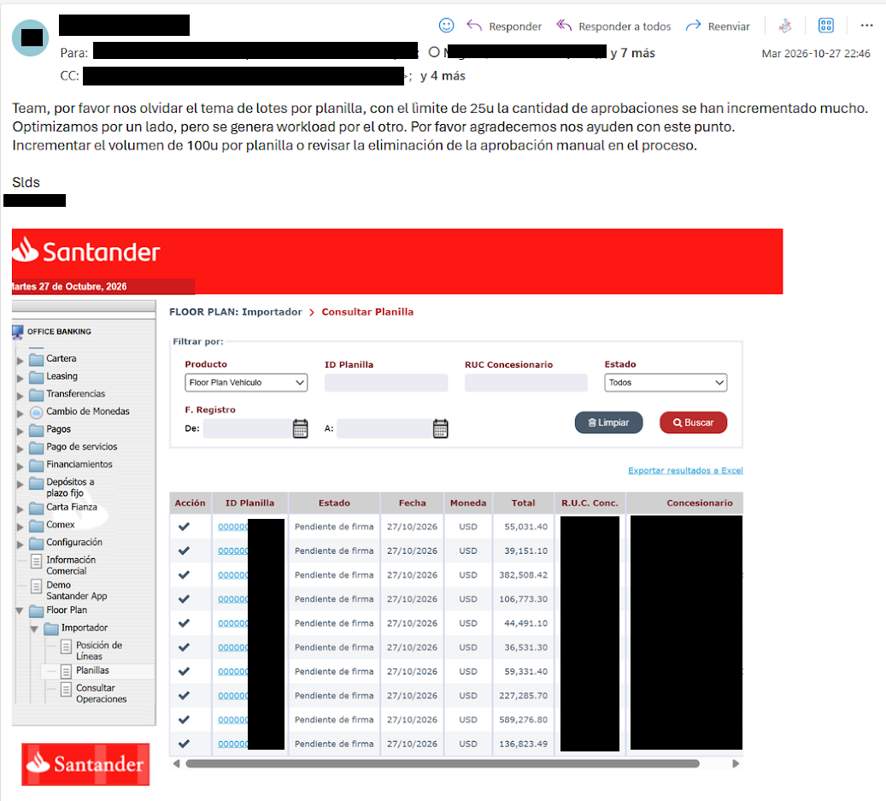
\includegraphics[width=1.00\textwidth]{figuras/image22}
\caption{Solicitud a Santander para ampliar el límite de unidades por planilla y planillas pendientes de aprobación en el home banking}\label{fig:21}
\end{figure}

Al tratarse de dos entrevistados, uno por cada operación, los resultados reflejan la percepción de usuarios clave y no pueden generalizarse al conjunto de los usuarios; sin embargo, aportan una validación cualitativa de los beneficios estimados por parte de quienes conocen el proceso en detalle.

La guía de preguntas y el registro de las respuestas se incluyen en el Apéndice A.

\section{Resultados obtenidos}

El principal resultado es la eliminación de dos tareas manuales del proceso de facturación: la carga del saldo de crédito por concesionario y, en Perú, el armado del Excel para Santander. Según la estimación del Capítulo 5, esto representa un ahorro de aproximadamente 442 horas anuales entre ambos países.

\subsection{Resultados favorables}

La Tabla~\ref{tab:18} resume el ahorro anual estimado por actividad, comparando la situación anterior con la situación con el sistema.

\begin{longtable}[]{@{}
  >{\raggedright\arraybackslash}p{(\columnwidth - 6\tabcolsep) * \real{0.2501}}
  >{\raggedright\arraybackslash}p{(\columnwidth - 6\tabcolsep) * \real{0.2500}}
  >{\raggedright\arraybackslash}p{(\columnwidth - 6\tabcolsep) * \real{0.2500}}
  >{\raggedright\arraybackslash}p{(\columnwidth - 6\tabcolsep) * \real{0.2500}}@{}}
\caption{Ahorro anual estimado por actividad}\label{tab:18}\\
\toprule\noalign{}
\endfirsthead
\caption[]{Ahorro anual estimado por actividad (continuación)}\\
\toprule\noalign{}
\endhead
\bottomrule\noalign{}
\endlastfoot
\textbf{Actividad} & \textbf{Situación anterior} & \textbf{Situación con el sistema} & \textbf{Ahorro anual estimado} \\
Carga de saldo de crédito -- Chile & \textasciitilde3,3 min por concesionario, casi todos los días hábiles & Actualización automática desde Forum & \textasciitilde97,5 h \\
Carga de saldo de crédito -- Perú & \textasciitilde3,3 min por concesionario, casi todos los días hábiles & Actualización automática desde Santander & \textasciitilde86,3 h \\
Armado del Excel para Santander -- Perú & Más de 10 min por concesionario y facturación & Informe automático vía API REST & \textasciitilde258 h \\
\textbf{Total} & & & \textbf{\textasciitilde442 h} \\
\end{longtable}

A estos resultados cuantificables se suman beneficios cualitativos:

\begin{itemize}
\item \textbf{Reducción de errores de tipeo}: al no cargarse los saldos a mano, desaparece el riesgo de errores como un cero de menos, que podían provocar el rechazo de la facturación de una o varias unidades.
\item \textbf{Visibilidad del proceso}: el correo de lote completo evita que el usuario tenga que consultar repetidamente el estado de las unidades.
\item \textbf{Trazabilidad}: cada comunicación con el banco queda registrada por VIN, lo que permite auditar y reprocesar envíos fallidos. En Chile, esto reemplaza un esquema en el que detectar un envío fallido requería revisar procesos del servidor y consultar a la entidad.
\item \textbf{Unificación de la información de crédito}: CR08 concentra livianos y pesados, resolviendo la falta de información sobre qué concesionarios operan con ambos tipos.
\end{itemize}
\subsection{Resultados negativos y limitaciones}

\begin{itemize}
\item
  \textbf{Alta Dua File sigue dependiendo de una carga manual}: los datos de DUA y plazo en Perú se continúan ingresando por el usuario mediante Excel. Esto mantiene un paso manual en el proceso de Perú y condiciona el informe a Santander a que esa información esté cargada a tiempo.
\item
  \textbf{Ausencia de ambiente de pruebas en Santander}: las validaciones con esa entidad solo pueden hacerse en producción.
\item
  \textbf{Cobertura de pruebas desigual}: solo VH Connect tiene pruebas automatizadas; los cambios en VH Legacy dependen de validación manual.
\item
  \textbf{Monitoreo limitado}: VH Connect dispone de los logs de la aplicación en GCP, pero se trata de un registro general de toda la aplicación; no existen dashboards ni métricas específicas del proceso de informe a las entidades bancarias, y las alertas se limitan a las notificaciones a Microsoft Teams. Analizar un error puntual implica buscarlo dentro del log completo. En VH Legacy la situación es más restrictiva: el log disponible en OpenShift tiene una retención muy acotada (aproximadamente una hora de actividad), ya que los registros nuevos reemplazan a los anteriores, por lo que la información de un error se pierde si no se consulta a tiempo.
\item
  \textbf{Ahorro estimado, no medido}: las 442 horas surgen de tiempos relevados con los usuarios y de la actividad real registrada en la base de datos, pero no de una medición sistemática antes y después de la implementación. No obstante, el usuario referente indicó en la entrevista que con el proceso anterior se llegaban a perder ``horas semanales'', una apreciación consistente con la estimación.
\item
  \textbf{Control manual residual}: aunque los usuarios consideran confiable el saldo actualizado automáticamente, el equipo continúa verificándolo habitualmente contra el home banking, lo que indica que la confianza en el sistema todavía está en construcción en esta etapa inicial de uso.
\item
  \textbf{Errores detectados en producción}: durante la validación con Santander se detectó que los importes con un solo decimal eran interpretados con la coma desplazada (por ejemplo, 28123,10 se registraba como 2812,31), debido a una regla de formato no documentada por la entidad. El detalle se presenta en la sección \textbf{Problemas detectados durante la integración.}
\end{itemize}

\section{Síntesis del capítulo}

Los resultados muestran que la integración con las APIs de Forum y Santander permite automatizar la actualización del crédito disponible y el informe de facturas, dos tareas que hasta ahora se realizaban de forma manual y con riesgo de error. El ahorro estimado ronda las 442 horas anuales entre Chile y Perú, acompañado de mejoras en trazabilidad y visibilidad del proceso. Además, la participación de los usuarios permitió ajustar la solución durante su implementación, y las entrevistas realizadas confirmaron cualitativamente los beneficios estimados, en particular la reducción de errores de carga y la visibilidad que aporta el correo de despacho.

Al mismo tiempo, el trabajo evidencia limitaciones: la carga de DUA y plazo en Perú sigue siendo manual; Santander no ofrece un ambiente de pruebas, lo que llevó a detectar errores de formato recién en producción; la cobertura de pruebas automatizadas se limita a VH Connect; el monitoreo depende de logs generales, con una retención muy acotada en VH Legacy; y los beneficios de tiempo son estimaciones y no mediciones. Estos puntos se retoman en el Capítulo 8 como parte de las conclusiones y de las recomendaciones para futuras líneas de trabajo.
